\section{Family ties between 1523 and 1680}
During the timeperiod between 1520 and 1680 there were 257 men active in the Council of the Realm. As discussed earlier in subchapter \ref{councilofrealm} the council consisted mostly of men with noble background. To quantify this: according to the dataset 236 of the 257 councillors (91.8\%) were part of the ancient nobility "uradel", and only approximately 5\% were of unknown or ignoble background, most of the time bishops or other clerics.  

\begin{table}
	\caption{Absolute amount in different ranks}
	\centering
	\begin{tabular}{cccccc}
		\hline
		Commoner & Ennobled & Estate unknown & Unknown & Ancient nobility & \\
		\hline
		5 & 8 & 7 & 1 & 236 & = 257 \\
		\hline
	\end{tabular}
	\caption{Proportional amount in different ranks (rounded)}
	\centering
	\begin{tabular}{cccccc}
		\hline
	    Commoner & Ennobled & Estate unknown & Unknown & Ancient nobility & \\
	    \hline
	    1.9 & 3.1 & 2.7 & 0.3 & 91.8 & \% \\
	\end{tabular}
\end{table}

The kingdom of Sweden was ruled by nine monarchs: Gustavus Vasa (1523-1560), Eric XIV (1560-1568), Johan III (1568-1592), Sigismund (1592-1599), Charles IX (1599-1611), Gustavus Adolphus (1611-1632), Christina (1644-1654), Carl X Gustav (1654-1660) and Carles XI (1672-1697), and two regnants from 1632 to 1654 and from 1660 to 1672 during the timeperiod. The amount of councillors appointed by each monarch or regnant varied from none to 56. Yet, 13 councillors were present before the regin of Gustavus Vasa.

The monarchs who appointed the most councillors were Gustavus Vasa (56) and queen Christina (45). The large number of councillors appointed by Gustavus Vasa may be explained by the sheer length of his regin. He ruled Sweden for 37 years, whereas all of the other monachs ruled less than 20 years. Also the religious Reformation was perfromed during his regin. Probably the bishops and clerics that lost their position in the Council were replaced by noblement chosen by the monarch. As queen Christina ruled only for ten years, the exceptionally high number on her regin is interesting. Her regin will be discussed in greater detail in subchapter \ref{christina}. 

Why king Sigismud did not appoint any new councillors? 

\begin{figure}
	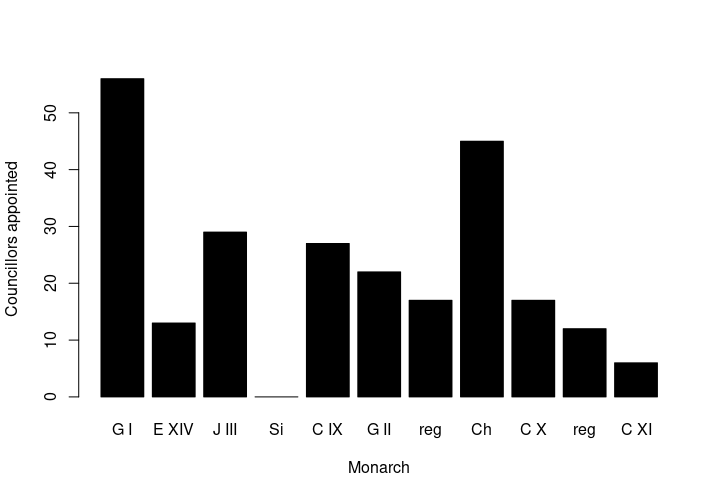
\includegraphics[scale=0.6]{councillorspermonarch.png}
	\centering
	\caption[Number of councillors appointed by each ruler between 1523-1680] {Number of councillors appointed by each monarch or regnant from 1523 to 1680. (\cite{councillorsDS})} 
	\centering
\end{figure}

All of the councillors between 1520 and 1680 are represented in a graph of 257 nodes and 362 edges, with self loops and parallel edges removed. The number of edges exceeds the number of nodes which means that theoretically all of the nodes could be linked to another one. However, the edges are not distributed that way. Some of the nodes are linked to more than one other nodes, but some isolated nodes are indeed present. The average degree of the graph is 2.817 $\approx$ 2.8 meaning that councillors typically had 2 or 3 direct relations to the prior member of the Council.

The graph density is 0.011. In the mathematical definition the graph is sparse (scale from 0 to 1). However, interpretation in practical sense is not that straightforward. Having a completely dense social network, meaning that every node is directly linked to everyone else is almost impossible. In this context it would mean, that each councillor is a direct relative through blood or marriage to each other, which would be weird to say at least. Further taking the dimension of time into account the mathematical interpretation would be even more nonsensical, how a nobleman appointed to the council in the 1670's could be directly linked to a bishop died in 1530's. 

The question wheither or not the councillors were higly linked to each other is more of a qualitative one. And probably the graph density has more explanatory value as a parameter to be compared between networks or in the graphs depicting shorter time intervals. 

The most interesting part is the nodes with the highest and lowest degree. Maybe the most eclectic and fascinating group is the isolated nodes. There are 33 isolated nodes meaning that 33 councillors did not have any family ties within the Council. Some of them are members of the nobility with family ties to councillors prior the beginning year of the dataset, so, the connections are not present in this graph. These are for example: Ture Bengtsson Lilliesparre (127) or Nils Olofsson Vinge (242). Some of the isolated nodes represent bishops and clerics like Magnus Sommar (186) or Ingemar Petri (162). 

The isolated nodes also tells about the international relationships during the timeperiod. For example a French teacher Dionysius Beurraeus or a Scottish baron Robert Douglas can be found. Also German Conrad von Pyhy is mentioned.
For example king Gustavus Adolpus' illegitimate son Gustaf Gustafsson af Vasaborg (241) can be found on the Council. 

The nodes with the highest degree ($\geq$ 5) are of councillors who are part of the old well known aristocratic families like De la Gardie, Oxentierna, Gyllenstierna, Bielke, Stenbock, Sparre and Ribbing. Also Finnish families of Horn and Kurck can be found. 

\subsection{Prior 1600}
The graph of councillors prior the violent years 1600 and 1601 consist of 111 nodes and 92 edges. 

The average degree in this graph is 1.658 $\approx$ 1.7, meaning that typically councillors were directly related to one or two other members. The number is smaller than in the larger graph. However, it can also be explained by the fact that the edges have not been cumulated as mutch as in the larger graph. Maybe the closest comparison is the graph of councillors family ties post 1601.

The graph density is 0.015, a slightly higher than in the larger graph. 

The amount of isolated nodes is significant: 26, as in the larger graph it was 33. The fact that, all of the bishops and clerics must be present in this graph, partly explains this. Limiting the time range also breaks some of the existing links, so for example Pontus De la Gardie seems to be without any connections in that graph even though his descendands were remarkably woven into the networks of Swedish aristocracy. Taking these factors into account, still the relatively high number of isolated nodes may tell about the relatively high number of "newcomers" and further social mobility.

The nodes with highest degree ($\geq$ 4) were of the remarkable noble families such as Bielke and Stenbock, however the Bååt family is more apparent in that graph than in the larger one or any of the later ones (TODO check). Did something happen to them?

In fact the last councillor to be executed in Sweden was in 1605.%TODO 

\subsubsection{the Last Man Standing: Nils Gyllenstierna}
\subsection{Post Duke Charles' revenge}
In year 1602 duke Charles had to appoint new councillors.

The graph of councillors post year 1601 consists of 146 nodes and 184 edges, again, the number of edges exceeds the number of nodes. After 1601 the average degree of node is 2.251 $\approx$ 2.3, larger than the 1.7 prior 1600. Visually the graph seems more dense. 

The number of isolated nodes is significantly lower: 16, again it must be remembered that limiting the time range removes some existing family ties. Bååt was along them.

Overall it seems that the family affiliations became more important in the 17th century than before.

\subsection{In the Court of Queen Christina}
The graph is so small that it is not entierly comparable to the other ones.

Rosenhane who gave the Hortus Regius book
\begin{figure}
	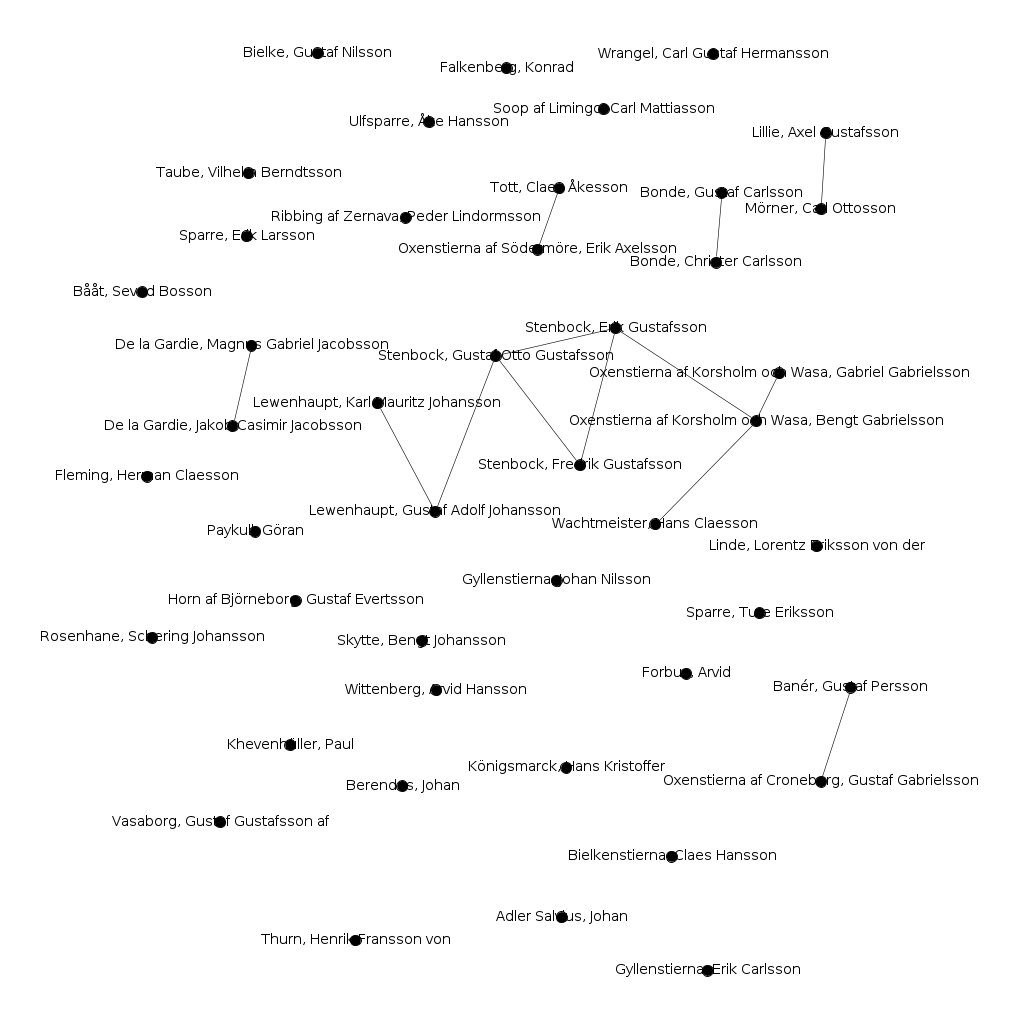
\includegraphics[width=\linewidth]{councillors_1644-1654.png}
	\caption[Councillors appointed by queen Christina]{A graph of councillors appointed by queen Christina between 1644 and 1654.(\cite{councillorsDS})} 
	\centering
\end{figure}

\label{christina}